\documentclass{beamer}
\usepackage{pgfpages}

%\setbeameroption{show notes on second screen=right}

\usepackage[utf8]{inputenc} 
\usepackage[T1]{fontenc}
\usepackage{beamerthemesplit}
\usepackage{graphicx}
\usepackage{tabularx}
\usepackage{forest}
\usepackage{pifont}
\usepackage{multirow}
%\usepackage{movie15}

\newcommand{\cmark}{\ding{51}}%
\newcommand{\xmark}{\ding{55}}

\DeclareMathOperator*{\argmin}{argmin}
\DeclareMathOperator*{\argmax}{argmax}


\title{Automated Place Detection Based on Coherent Segments}
\author{Mahmut Demir and H. Isil Bozma}
\institute{Intelligent Systems Laboratory \\
Electrical and Electronics Engineering, Boğaziçi University, Istanbul, Turkey}
\vspace{-1cm}

%\date[ICCV]{ICCV 2015 International Conference on Computer Vision }
\titlegraphic{\includegraphics[width=20mm]{img/conf_logo.png} \\ \includegraphics[width=6mm]{img/master/isllogo2.JPG}\hspace*{1cm}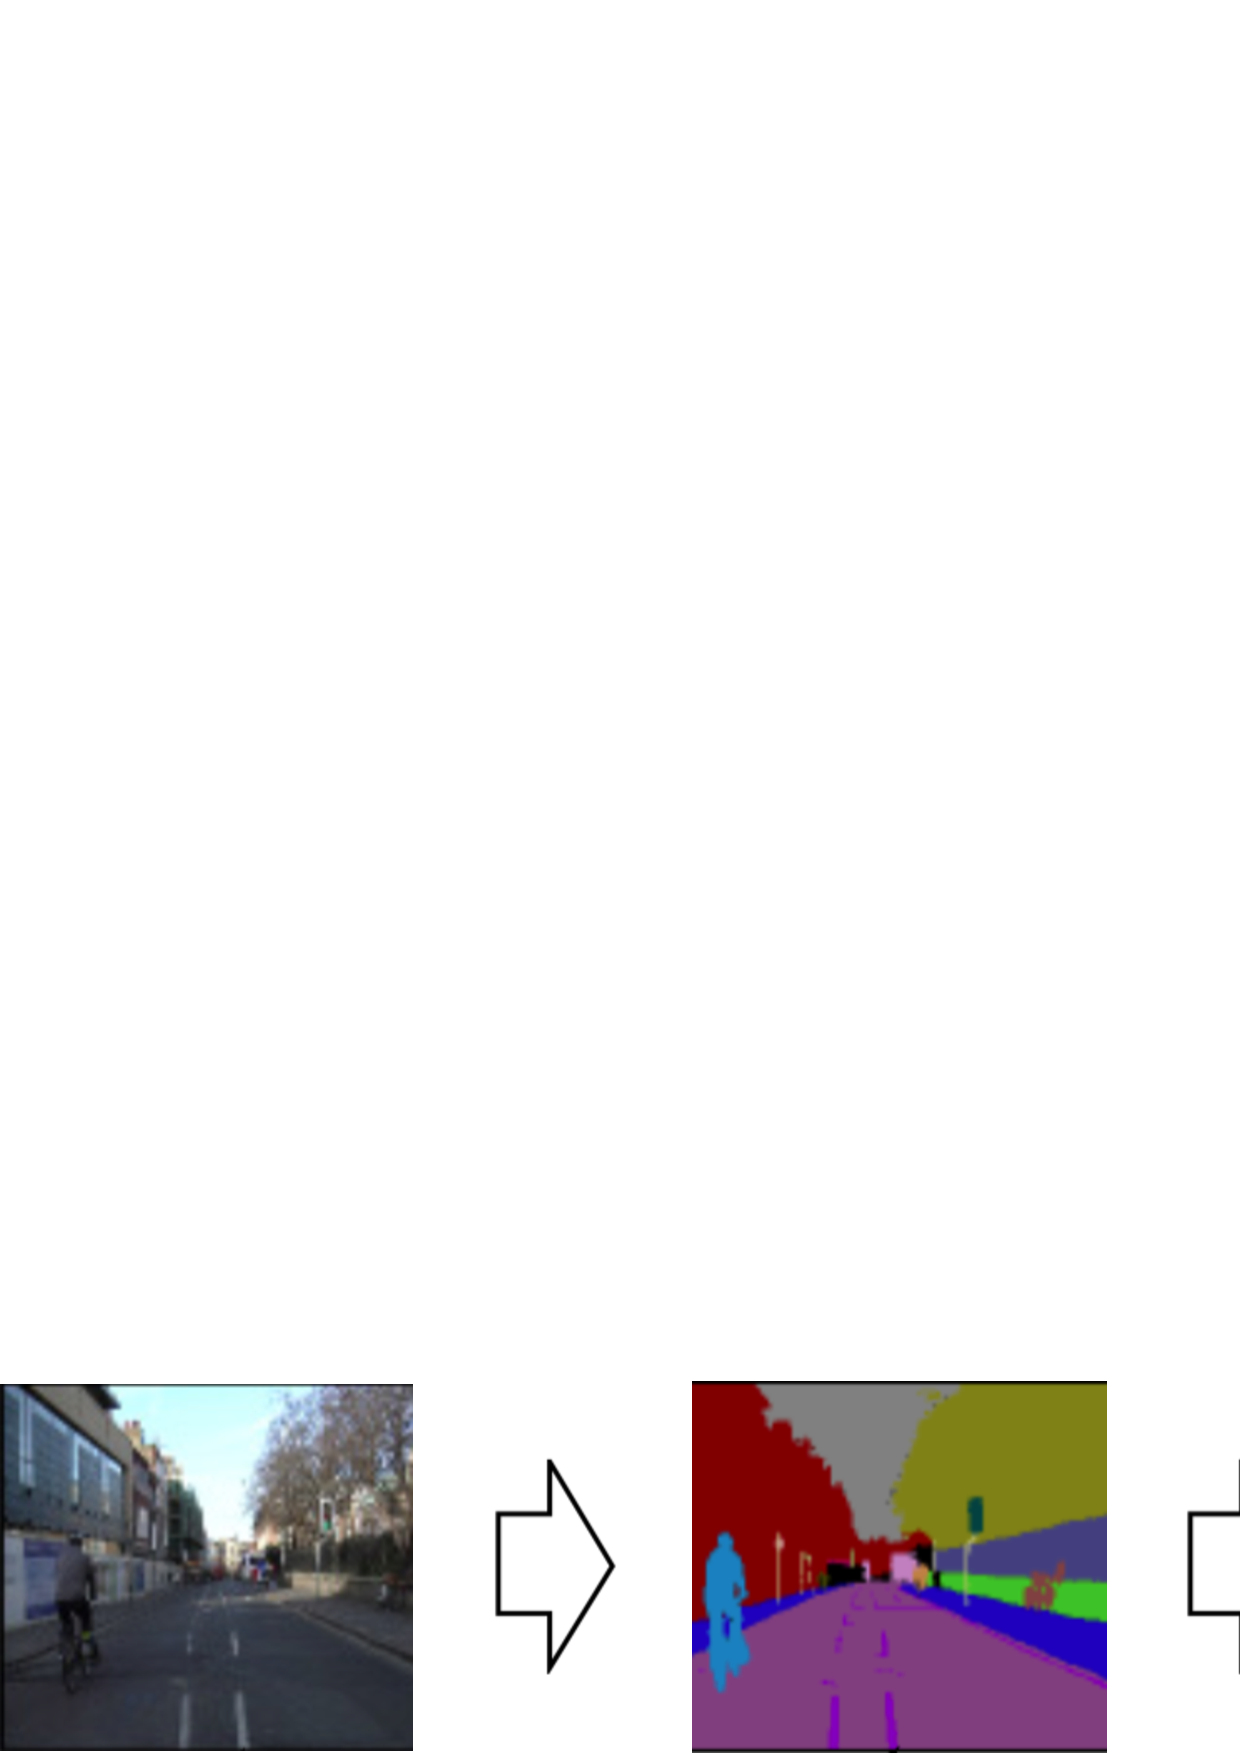
\includegraphics[width=30mm]{img/master/cover}\hspace*{1cm}\includegraphics[width=6mm]{img/master/bu2.JPG}}
\begin{document}


\frame{\titlepage}

\section[Overview]{}
\frame{\tableofcontents}

%DEF.TEX: DEFINITIONS HEADER FILE

%GENERAL DEFINITIONS
%-------------------
\newcommand{\cspace}{\vspace{0.2in}}
\newcommand{\beqn}{\begin{eqnarray*}}
\newcommand{\eeqn}{\end{eqnarray*}}
\newcommand{\defeq}{\stackrel{\triangle}{=}}
\newcommand{\cbox}{\Box}

%sets, vectors
%-------------
\newcommand{\cc}{c}
\newcommand{\ce}{e}
\newcommand{\ck}{k}
\newcommand{\cp}{p}
\newcommand{\cq}{q}


\newcommand{\cK}{\mathcal K}
\newcommand{\cS}{\mathcal S}
\newcommand{\cM}{\mathbf M}
\newcommand{\cP}{\mathcal P}
\newcommand{\cE}{\mathit E}
\newcommand{\cX}{\mathcal X}
\newcommand{\cI}{\mathcal I}
\newcommand{\cC}{\mathcal C}
\newcommand{\cN}{\mathcal N}
\newcommand{\cV}{\mathcal V}
\newcommand{\cA}{{\mathcal{A}}}
\newcommand{\cF}{{\mathcal{F}}}
\newcommand{\cD}{{\mathcal{D}}}




\newcommand{\cb}{b}
\newcommand{\cd}{d}
\newcommand{\cg}{g}
\newcommand{\crho}{\rho}
\newcommand{\eps}{\varepsilon}



\newcommand{\Ip}{\cI_{2 \cp}}

\newcommand{\cT}{T}

\newcommand{\ccr}{r} % \cr is reserved 
\newcommand{\rp}{\ccr'}
\newcommand{\rr}{\ccr \rp}
\newcommand{\drr}{\cd_{\rr}}
\newcommand{\drrh}{\hat{\cd}_{\rr}}
\newcommand{\crr}{\cc_{\rr}}
\newcommand{\cz}{z}
\newcommand{\zp}{\cz'}
\newcommand{\zz}{\cz \zp}
\newcommand{\dzz}{\cd_{\zz}}
\newcommand{\czz}{\cc_{\zz}}
\newcommand{\dzzh}{\hat{\cd}_{\zz}}

\newcommand{\boldN}{{\mathbb Z}^+}
\newcommand{\boldR}{\mathbb{R}}
\newcommand{\gamb}{(\cgamma^k+\cbeta)}

%navigation function
%-------------------
\newcommand{\cdelta}{\delta}
\newcommand{\csigma}{\sigma}
\newcommand{\calpha}{\alpha}
\newcommand{\cbeta}{\beta}
\newcommand{\cgamma}{\gamma}
\newcommand{\cphi}{\varphi}
\newcommand{\hphi}{\hat{\cphi}}
\newcommand{\dphi}{\nabla \cphi}
\newcommand{\dhphi}{\nabla \hphi}
\newcommand{\dgamma}{\nabla \cgamma}
\newcommand{\dbeta}{\nabla \cbeta}
\newcommand{\ddphi}{D^2 \cphi}
\newcommand{\ddhphi}{D^2 \hat{\cphi}}
\newcommand{\ddgamma}{D^2 \cgamma}
\newcommand{\ddbeta}{D^2 \cbeta}
\newcommand{\crit}[1]{{{\cC}_{#1}}}

\newcommand{\conv}[1]{\left( \cI_2 \otimes \cc_{{#1}} \right)}
\newcommand{\convT}[1]{\left( \cI_2 \otimes \cc_{{#1}}^T \right)}
\newcommand{\conve}[1]{\left( \cI_2 \otimes \ce_{{#1}} \right)}
\newcommand{\conveT}[1]{\left( \cI_2 \otimes \ce_{{#1}}^T \right)}
\newcommand{\dbetac}[1]{\cd_{{#1}}^T \convT{{#1}}}

%\newcommand{\ei}{\ce_i}
\newcommand{\ej}{\ce_j}
\newcommand{\en}{\ce_n}
\newcommand{\el}{\ce_l}
%\newcommand{\bi}{\cb_i}
\newcommand{\bj}{\cb_j}
\newcommand{\bl}{\cb_l}
\newcommand{\bn}{\cb_n}
%\newcommand{\bm}{\cb_m}
\newcommand{\bz}{\cb_{\cz}}
\newcommand{\gi}{\cg_i}
\newcommand{\gj}{\cg_j}
\newcommand{\gn}{\cg_n}
\newcommand{\gl}{\cg_l}
\newcommand{\dij}{\cd_{ij}}
\newcommand{\dji}{\cd_{ji}}
\newcommand{\dln}{\cd_{ln}}
\newcommand{\dil}{\cd_{il}}
\newcommand{\din}{\cd_{in}}
\newcommand{\dli}{\cd_{li}}
\newcommand{\dni}{\cd_{ni}}
\newcommand{\gij}{\cg_{ij}}
\newcommand{\gln}{\cg_{ln}}
\newcommand{\cij}{\cc_{ij}}
\newcommand{\cln}{\cc_{ln}}
\newcommand{\betaij}{\cbeta_{ij}}
\newcommand{\betaln}{\cbeta_{ln}}
\newcommand{\betaoi}{\cbeta_{0i}}
\newcommand{\betaoj}{\cbeta_{0j}}
\newcommand{\betaol}{\cbeta_{0l}}
\newcommand{\betaon}{\cbeta_{0n}}
\newcommand{\alij}{\calpha_{ij}}
\newcommand{\alln}{\calpha_{ln}}
\newcommand{\alil}{\calpha_{il}}
\newcommand{\alin}{\calpha_{in}}
\newcommand{\alli}{\calpha_{li}}
\newcommand{\alni}{\calpha_{ni}}
\newcommand{\aloi}{\calpha_{0i}}
\newcommand{\aloj}{\calpha_{0j}}
\newcommand{\alon}{\calpha_{0n}}
\newcommand{\alol}{\calpha_{0l}}
\newcommand{\sigmaij}{\csigma_{ij}}
\newcommand{\sigmaln}{\csigma_{ln}}
\newcommand{\sigmaoi}{\csigma_{0i}}
\newcommand{\sigmaoj}{\csigma_{0j}}
\newcommand{\dbetaij}{\dbeta_{ij}}
\newcommand{\dbetaln}{\dbeta_{ln}}
\newcommand{\dbetaoi}{\dbeta_{0i}}
\newcommand{\dbetaoj}{\dbeta_{0j}}
\newcommand{\ddbetaij}{\ddbeta_{ij}}
\newcommand{\ddbetaln}{\ddbeta_{ln}}
\newcommand{\magbetaij}{\| \nabla \betaij  \|}
\newcommand{\magbetaln}{\| \nabla \betaln  \|}

%indices, summation, product
%---------------------------
\newcommand{\iinP}{i \in \cP}
\newcommand{\kinK}{k \in \cK}
\newcommand{\iinS}{i \in \cS}
\newcommand{\ijinS}{i,j \in \cS}
\newcommand{\jinP}{j \in \cP}
\newcommand{\ninP}{n \in \cP}
\newcommand{\ninS}{n \in \cS}
\newcommand{\minP}{m \in \cP}
\newcommand{\rinP}{r \in \cP}
\newcommand{\ijinQ}{(i,j) \in \cQ}
\newcommand{\lninQ}{(l,n) \in \cQ}
\newcommand{\ijinQo}{(i,j) \in \Qo}
\newcommand{\lninQo}{(l,n) \in \Qo}
\newcommand{\prij}{\prod_{\ijinQ}}
\newcommand{\prln}{\prod_{\lninQ}}
\newcommand{\prijo}{\prod_{\ijinQo}}
\newcommand{\prlno}{\prod_{\lninQo}}
\newcommand{\pri}{\prod_{\iinP}}
\newcommand{\prj}{\prod_{\jinP}}
\newcommand{\sumi}{\sum_{\iinP}}
\newcommand{\sumiS}{\sum_{\iinS}}
\newcommand{\sumj}{\sum_{\jinP}}
\newcommand{\sumn}{\sum_{\ninP}}
\newcommand{\summ}{\sum_{\minP}}

\newcommand{\sumij}{\sum_{\ijinQ}}
\newcommand{\sumln}{\sum_{\lninQ}}
\newcommand{\sumijln}{\sumij \sumln^{(l,n) \neq (i,j)}}
\newcommand{\sumlnij}{\sumln \sumij^{(i,j) \neq (l,n)}}
\newcommand{\sumijo}{\sum_{\ijinQo}}
\newcommand{\sumlno}{\sum_{\lninQo}}
\newcommand{\sumijlno}{\sumijo \sumlno^{(l,n) \neq (i,j)}}
\newcommand{\sumlnijo}{\sumlno \sumijo^{(i,j) \neq (l,n)}}

\newcommand{\delij}{\cdelta_{ij}}
\newcommand{\delln}{\cdelta_{ln}}
\newcommand{\delin}{\cdelta_{in}}
\newcommand{\delil}{\cdelta_{il}}
\newcommand{\delni}{\cdelta_{ni}}
\newcommand{\delli}{\cdelta_{li}}
\newcommand{\deltaij}{\cdelta^2_{ij}}
\newcommand{\deltaln}{\cdelta^2_{ln}}
\newcommand{\rhoo}{\crho_0}
\newcommand{\rhoi}{\crho_i}
\newcommand{\rhoj}{\crho_j}
\newcommand{\rhol}{\crho_l}
\newcommand{\rhon}{\crho_n}
\newcommand{\rhooi}{\crho_{0i}}
\newcommand{\rhooj}{\crho_{0j}}
\newcommand{\rhool}{\crho_{0l}}
\newcommand{\rhoon}{\crho_{0n}}
\newcommand{\rhoij}{\crho_{ij}}
\newcommand{\rholn}{\crho_{ln}}
\newcommand{\rhomin}{\crho'}
\newcommand{\rhomino}{\crho''}
\newcommand{\rhomax}{\crho_{max}}
\newcommand{\gammamax}{\cgamma_{max}}
\newcommand{\forij}{\forall \ijinQ}
\newcommand{\forln}{\forall \lninQ}
\newcommand{\forijo}{\forall \ijinQo}
\newcommand{\fori}{\forall \iinP}
\newcommand{\fork}{\forall \kinK}
\newcommand{\forj}{\forall \jinP}
\newcommand{\forn}{\forall \ninP}
\newcommand{\form}{\forall \minP}
\newcommand{\forr}{\forall \rinP}
\newcommand{\foriS}{\forall \iinS}

%Partitioning of the free space
%------------------------------
\newcommand{\Fzero}{\cF_1(\eps)}
\newcommand{\Fone}{\cF_0(\eps)}
\newcommand{\Ftwo}{\cF_2(\eps)}

%Outer Boundary
%---------------
\newcommand{\mbi}{\| \bi \|}
\newcommand{\mgi}{\| \gi \|}


%Hessian
%-------
\newcommand{\cL}{L}
\newcommand{\Lo}{\cL_0}
\newcommand{\Lone}{\cL_1}
\newcommand{\Lij}{\cL_{ij}}
\newcommand{\Loi}{\cL_{0i}}
\newcommand{\Loj}{\cL_{0j}}
\newcommand{\co}{o}
\newcommand{\Qo}{\cQ^0}

%Non-degeneracy
%---------------
\newcommand{\Lrr}{\cL_{\rr}}
\newcommand{\deltarr}{\cdelta^2_{\rr}}
\newcommand{\rhorr}{\crho_{\rr}}
\newcommand{\betarr}{\cbeta_{\rr}}
\newcommand{\cB}{B}
\newcommand{\ctheta}{\theta}
\newcommand{\cR}{R}
\newcommand{\cRt}{\cR_{\ctheta}}
\newcommand{\vr}{\drrh \otimes \ce_{\ccr}}
\newcommand{\vrt}{\cRt \drrh \otimes \ce_{\ccr}}
\newcommand{\costh}{\cos^2 \ctheta}

%Polarity
%---------

\newcommand{\cs}{s}
\newcommand{\Qp}{\cQ'}
\newcommand{\Pp}{\cP'}
\renewcommand{\Pi}{\cP_i}
\newcommand{\Pj}{\cP_j}
\newcommand{\bzp}{\cb_{\zp}}
\newcommand{\Pz}{\cP_{\cz}}
\newcommand{\Qz}{\cQ_{\cz}}
\newcommand{\Qzp}{\Qz^*}
\newcommand{\pz}{\cp_{\cz}}
\newcommand{\iinPz}{i \in \Pz}
\newcommand{\jinPz}{j \in \Pz}
\newcommand{\linPz}{l \in \Pz}
\newcommand{\ninPz}{n \in \Pz}
\newcommand{\ijinQz}{(i,j) \in \Qz}
\newcommand{\lninQz}{(l,n) \in \Qz}
\newcommand{\sumiz}{\sum_{\iinPz}}
\newcommand{\sumjz}{\sum_{\jinPz}}
\newcommand{\sumlz}{\sum_{\linPz}}
\newcommand{\sumnz}{\sum_{\ninPz}}
\newcommand{\sumijz}{\sum_{\ijinQz}}
\newcommand{\sumlnz}{\sum_{\lninQz}}
\newcommand{\sumlnzp}{\sum_{\lninQz'}}
\newcommand{\sumlnzpp}{\sum_{\lninQz''}}
\newcommand{\PzP}{(i,j) \in \Qzp}
\newcommand{\ccN}{N}
\newcommand{\Neps}{\ccN}
\newcommand{\cw}{w}
\newcommand{\cm}{m}
\newcommand{\cn}{n}
\newcommand{\cx}{x}
\newcommand{\cLambda}{\Lambda}
\newcommand{\cJ}{J}
\newcommand{\cG}{\bar{g}}
\newcommand{\gz}{\cG_{\cz}}
\newcommand{\cv}{v}
\newcommand{\vz}{v_{\cz}}
\newcommand{\vn}{\sum_{\ninP_{\cz}} \cJ ( \cb_n - \cG_{\cz} ) \otimes \ce_n}
\newcommand{\cell}{r}
\newcommand{\tw}{w}
\newcommand{\ninPp}{n \in \Pp}
\newcommand{\Sigmas}{\Sigma^+}
\newcommand{\csig}{\sigma^+}
\newcommand{\gija}{\|\gij\|}
\newcommand{\glna}{\|\gln\|}
\newcommand{\cDel}{\Delta}
\newcommand{\cLam}{\Lambda}
\newcommand{\Dz}{\cDel_{\cz}}
\newcommand{\Lz}{\cLam_{\cz}}


%Temporary variables
%-------------------
\newcommand{\ccw}{w}
\newcommand{\ccu}{u}
\newcommand{\ccv}{v}
\newcommand{\ccy}{y}
\newcommand{\ccx}{x}
\newcommand{\cpsi}{\psi}







		%\multirow{2}{*}{{\textcolor{green}{\cmark}}} &  1) Improved localization error with  decreased denseness sensitivity \\
		%& 2) No need for sequential imaging 
		%\end{tabular}
\section{Introduction}
\subsection{Problem definition}
\frame
{
	\frametitle{Introduction}
	
	\begin{columns}[t,onlytextwidth]
		\hspace*{-1cm}
		
		\column{.99\textwidth}
		\vspace{-0.5cm}
		\begin{itemize}
			\item Goal: Automated appearance-based place detection 
			\item Place is a specific spatial unit or area  
			\item Place detection is a prior step to
			\begin{itemize}
				\item Place recognition
				\item Topological mapping
				\item Semantic scene understanding
			\end{itemize}
		\end{itemize}
	\end{columns}
}
\frame
{
	\frametitle{Introduction}
	
	\begin{columns}[t,onlytextwidth]
		\hspace*{-1cm}
		
		\column{.99\textwidth}
		\vspace{-0.5cm}
		\begin{itemize}
			\item Appearance-based approach
			\begin{itemize}
				\item Suitable for scene content analysis 
				\item Geometric or odometric data may not be avaiable
			\end{itemize}
			\item Challenges
			\begin{itemize}
				\item Appearance variability
				\item Indiscriminate boundaries
			\end{itemize}
		\end{itemize}
	\end{columns}
}
\subsection{Related work}
\frame
{
	\frametitle{Introduction}
	
	\begin{columns}[t,onlytextwidth]
		\hspace*{-1cm}
		
		\column{.99\textwidth}
		\vspace{-0.5cm}
		\begin{itemize}
			\item Related work
			\begin{itemize}
				\item Partioning of incoming sensory data based on similarity
				\item Clustering
				\item Feature types:
				\begin{itemize}
					\item Global: Histograms, Census Transform, GIST \textcolor{red}{\xmark} ~Sensitive
					\item Local: SIFT, SURF \textcolor{red}{\xmark} ~Low level, Matching
					\item Hybrid: BoW, Bubble Space \textcolor{red}{\xmark} ~Low level
				\end{itemize}
			\item Detecting transition regions (i.e. doors, passages, corridors) \textcolor{red}{\xmark} ~Fails if transitions are not obvious 
				
				
			\end{itemize}
			
		\end{itemize}
	\end{columns}
}
\subsection{Related work}
\frame
{
	\frametitle{Introduction}
	
	\begin{columns}[t,onlytextwidth]
		\hspace*{-1cm}
		
		\column{.99\textwidth}
		\vspace{-0.5cm}
		\begin{itemize}
			\item Proposed approach
			\begin{itemize}
				\item Visual segments
				\item Smooth body or head motion assumption
				\item Spatio-temporal coherence of visual segments
			\end{itemize}
			
			\item Advantages:
			\begin{itemize}
				\item More stable features
				\item Segments Summary Graphs representation
			\end{itemize}
			
		\end{itemize}
	\end{columns}
}
\subsection{General approach}
\frame
{
	\frametitle{General Approach}
	
	\begin{columns}[t,onlytextwidth]
		\hspace*{-1cm}
		
		\column{.99\textwidth}
		\vspace{-0.5cm}
		\begin{figure}[p]
			\centering
			\includegraphics[width = 0.9\textwidth]{img/icsc/diagram_approach}
		\end{figure}
		
	\end{columns}
}
\section{Method}
\subsection{Region Adjacency Graphs}
\frame
{
	\frametitle{Region Adjacency Graphs}
	
	\begin{figure}[p]
		\centering
		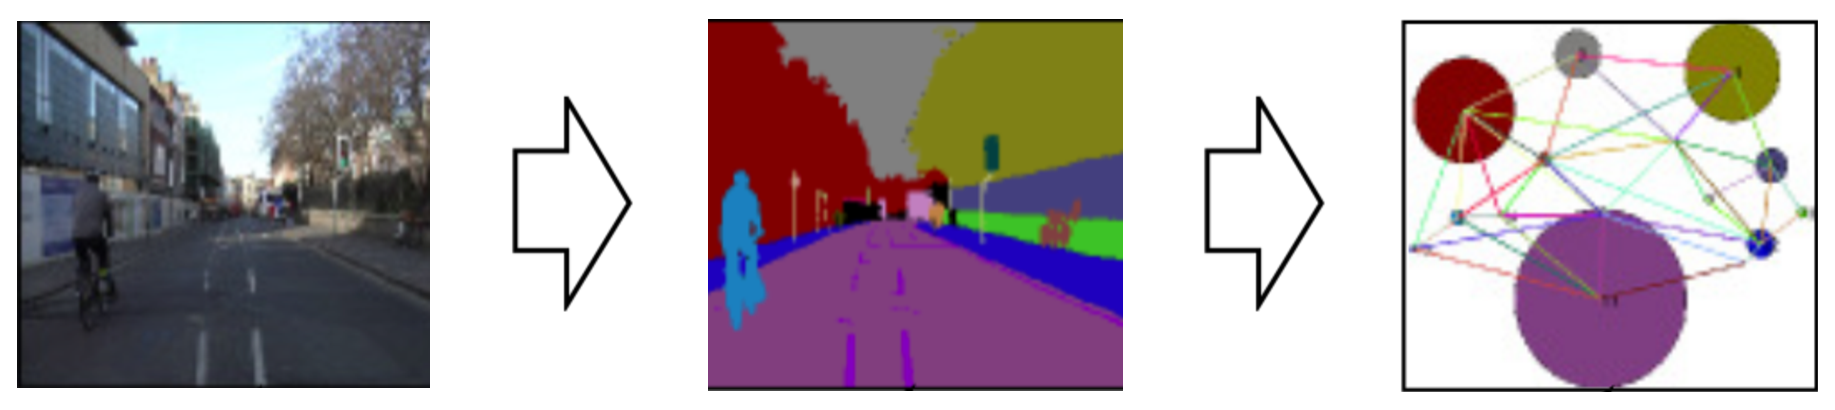
\includegraphics[width = 0.8\textwidth]{img/master/cover}
		\label{fig:rag}
	\end{figure}
	
	\begin{columns}[T]
		\column{.65\textwidth}
		\begin{itemize}
			\item Segments $\Rightarrow$ Nodes
			\item Spatial relations $\Rightarrow$ Edges
			\item Graph based segmentation method [Felzenszwalb, Huttenlocher, 2004]
		\end{itemize}
		
		
		\column{.4\textwidth}
		\vspace{-0.5cm}
		\begin{itemize}
			\item Nodes
			\begin{itemize}
				\item Color
				\item Position
				\item Size
			\end{itemize}
			\item Edges
			\begin{itemize}
				\item Mean color difference
			\end{itemize}
		\end{itemize}
	\end{columns}
	
}
\subsection{Temporal RAG Tracking}
\frame
{
	\frametitle{Temporal RAG Tracking}
	
	\begin{columns}[T]
		\hspace*{-1cm}
		\column{.55\textwidth}

		\begin{itemize}
			\item Matching consecutive RAGs:  
			\begin{itemize}
				\item Cost matrix $C^{kl}$ with $c_{ij} = \delta(s(\mathcal{N}^k_i),s(\mathcal{N}^l_j) )  $
				\item Optimal match by Hungarian method
				\item Remove nodes with matching cost > $\tau_m$
			\end{itemize}
			\item Nonmatched nodes - \\ Matching via backtracking
		\end{itemize}
		

		
		\column{.45\textwidth}

		
		\begin{figure}[p]
			\hspace*{-1.0cm}
			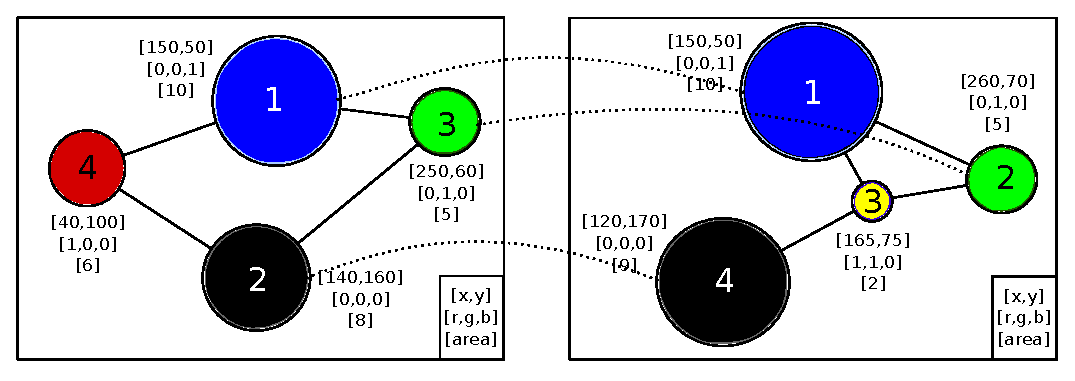
\includegraphics[width = 1.3\textwidth]{img/icsc/signature_graph.eps}
			\label{fig:signature_graph}
		\end{figure}
		\vspace*{-1.1cm}
		\begin{figure}[p]
			\hspace*{-2.5cm}
			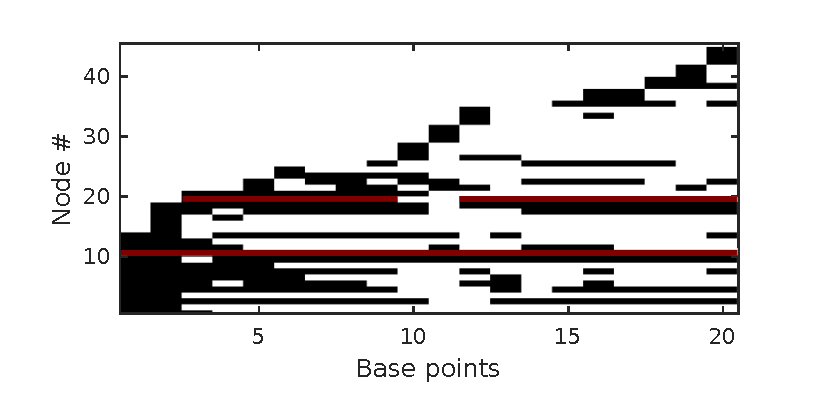
\includegraphics[width = 1.8\textwidth]{img/icsc/node_continuity.eps}
			\label{fig:rag_tracking}
		\end{figure}
		
	\end{columns} 
	
}
\subsection{Coherency score}
\frame
{
	\frametitle{Coherency score calculation}
		
	\begin{columns}[T]
	\column{.5\textwidth}
	\begin{itemize}
		\small
		\item Coherency over temporal window 
		\item Factors:
			\begin{itemize}
				\item $\tau_w$ - window size
				\item \# appearing nodes
				\item \# disappearing nodes
				\item node weights - $\rho^l_i$
			\end{itemize}
		\begin{figure}[p]
			\centering
			\hspace{-1cm}
			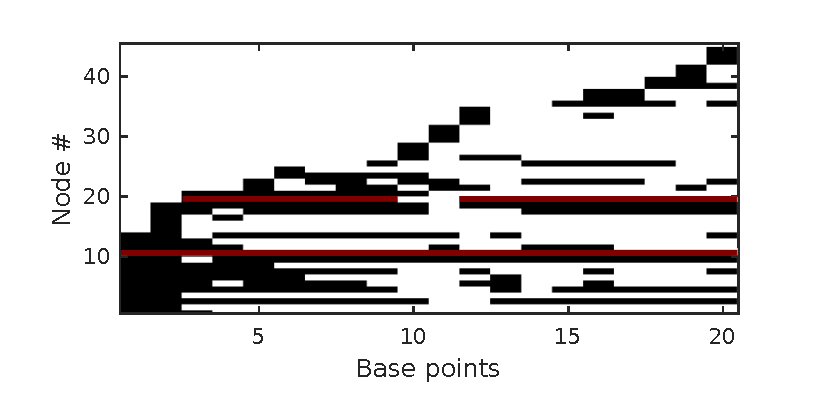
\includegraphics[width = 1\textwidth]{img/icsc/node_continuity.eps}
			\label{fig:coh_score_3}
		\end{figure}
	\end{itemize}
	\column{.6\textwidth}
	\hspace{-2cm}
	\small
	\begin{align}
	\varphi^k &= 1 - \sum\limits_{l=k-\tau_w}^{k}\sum\limits_{i=1}^{\lvert n^l \rvert}\rho^{l}_i (a^{l}_i + b^{l}_i) \label{eq:incoherency_score}	\end{align}
	where
	\begin{align}
%	a^l_i &= \begin{cases}
%	1 &\text{if }	M_{li}>0, \, M_{l-1,i}=0 \\
%	0 &\text{otherwise}
%	\end{cases}  \label{eq:a}	\\
%	b^l_i &= \begin{cases}
%	1 &\text{if }	M_{li}=0,  M_{l-1,i}>0 \\
%	0 &\text{otherwise}
%	\end{cases}  \label{eq:b}	\\
	\rho^l_i &\propto s_3(N^l_i) 
	\times \sum\limits_{k=l-{\tau_w}}^{l} M_{ki}>0 \label{eq:rho}									
	\end{align}

	\end{columns}
}
\subsection{Place Detection}
\frame
{
	\frametitle{Place Detection}
	
	\begin{columns}[t,onlytextwidth]
		\hspace*{-1cm}
		
		\column{.99\textwidth}
		\vspace{-0.5cm}
		\begin{figure}[p]
			\centering
			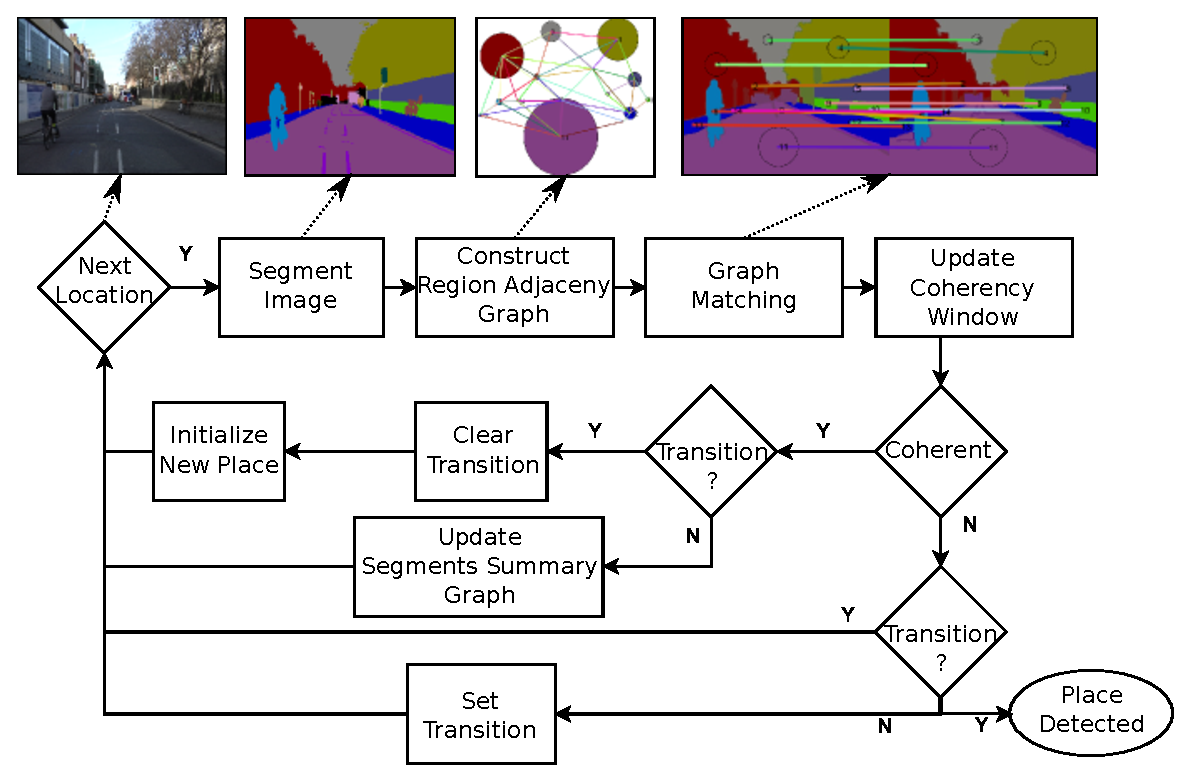
\includegraphics[width = 0.9\textwidth]{img/icsc/diagram}
		\end{figure}
		
	\end{columns}
}
\subsection{Segments Summary Graphs}
\frame
{
	\frametitle{Segments Summary Graphs}
	\begin{columns}[T]
	\column{1\textwidth}
		\begin{itemize}
			\item Contains apparent segments only
			\item Encodes spatial relations
		\end{itemize}
		\begin{figure}[p]
			\centering
			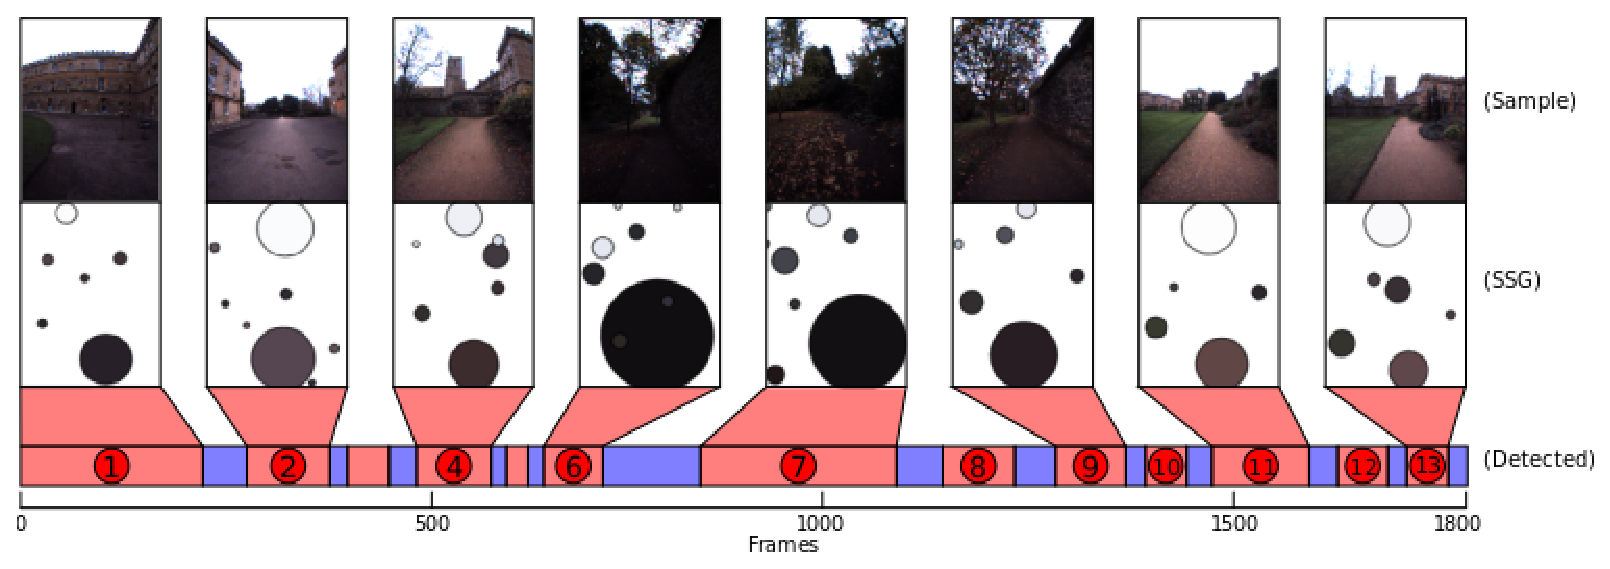
\includegraphics[width = 1.0\textwidth]{img/icsc/detected_places_nc.eps}
			\label{fig:ssg2}
		\end{figure}
	\end{columns}
	
}
\section{Experiments}
\frame
{
	\frametitle{Experiments}
	
	\begin{columns}[t,onlytextwidth]
		\hspace*{-1cm}
		
		\column{.99\textwidth}
		\vspace{-0.5cm}
		\begin{itemize}
			\item Outdoor [New College Dataset]
			\item Indoor [COLD Dataset] 
			\item Comparative study [VPC2009]
		\end{itemize}
	\end{columns}
}
\frame
{
	\frametitle{Outdoor experiments}
	
	
	\begin{columns}[T]
		\column{.65\textwidth}
		\begin{itemize}
			\item New College dataset
			\item 1800 basepoints 550 m
			\item Contains gradual changes
		\end{itemize}
		\centering
		\begin{figure}[p]
			\hspace{0.5cm}
			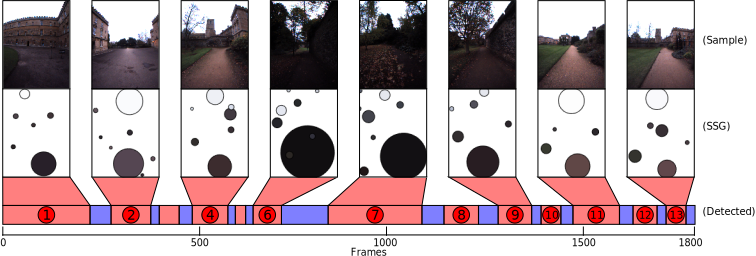
\includegraphics[width = 1\textwidth]{img/icsc/detected_places_nc}
			\label{fig:nc_ssg}
		\end{figure}

		\column{.35\textwidth}
		\centering New College Map
		\begin{figure}[p]
			\centering
			\hspace{0.5cm}
			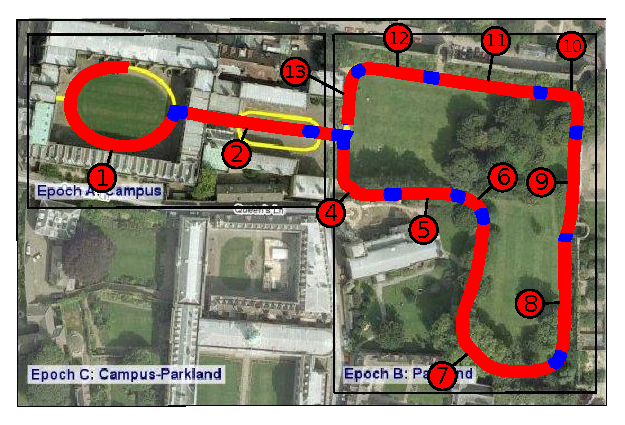
\includegraphics[width = 1.0\textwidth]{img/icsc/detected_places_nc_map}
			\label{fig:nc_map}
		\end{figure}
		

	\end{columns}		
	
}
\frame
{
	\frametitle{Indoor experiments}
	

	\begin{columns}[T]
		\column{.75\textwidth}
		
		\small
		\begin{itemize}
			\item Freiburg (Fr), Saarbrucken (Sa) and Ljubljana sites of COLD Dataset
		\end{itemize}
		\centering
		\begin{figure}[p]
			\centering
			\vspace{-0.5cm}
			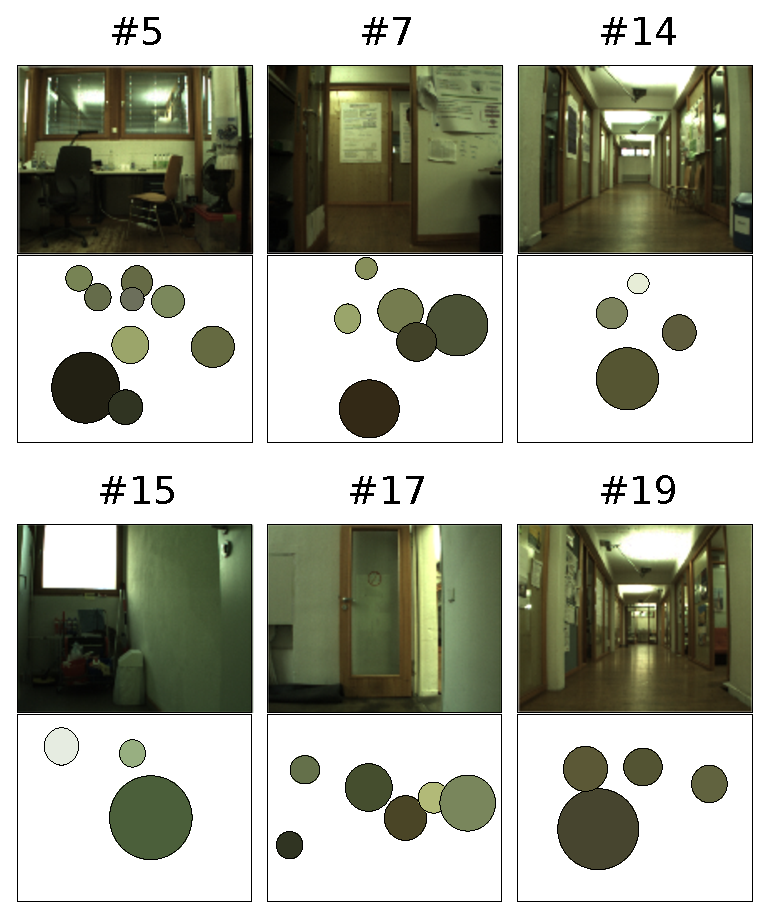
\includegraphics[width = 0.45\textwidth]{img/icsc/ssg-eval2}
			\label{fig:fr_ssg}
		\end{figure}
				
		\column{.25\textwidth}
		\begin{figure}[p]
			\centering Freiburg site
			\hspace{-0cm}
			\includegraphics[width = 1.0\textwidth]{img/icsc/detected_places_fr2_ssg}
			\label{fig:fr_map}
		\end{figure}
		

		
	\end{columns}		

}
\frame
{
	\frametitle{Comparison of Detected Places: SSG vs BD$^1$ (Bubble Descriptors) }
	
	\begin{columns}[T]
		\column{.5\textwidth}
		\small
		\centering
		SSG approach
		\vspace{-0.3cm}
		\begin{figure}[p]
			\centering
			\includegraphics[width = 0.5\textwidth]{img/master/detected_places_fr2_ssg.eps}
		\end{figure}
		\column{.5\textwidth}
		\small
		\centering
		BD approach
		\vspace{-0.3cm}
		\begin{figure}[p]
			\centering
			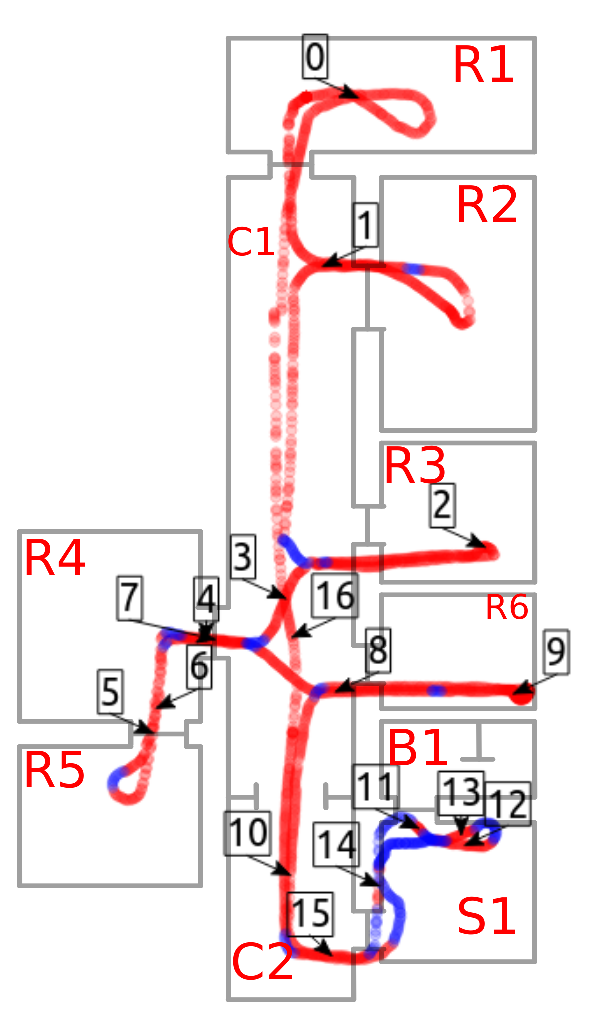
\includegraphics[width = 0.5\textwidth]{img/master/detected_places_fr2_bd.eps}
		\end{figure}
	\end{columns}
	
	\vspace*{2mm}	
	\noindent \textit{\tiny 1 - Karaoguz \& Bozma,  ICRA 2014, Autonomous Robots 2015	}
}
\frame
{
	\frametitle{VPC2009 Dataset}
	
	\begin{columns}[t,onlytextwidth]
		\hspace*{-1cm}
		
		\column{.99\textwidth}
		\vspace{-0.5cm}
		\small
		\begin{itemize}
			\item 21019 images from three different homes
			\item Challenging dateset:
			\begin{itemize}
				\item Unclear place boundaries
				\item Visual content varies
greatly with respect to the viewpoint due to small FOV
			\end{itemize}
			\item Comparison based on 43 manually annotated transition regions
			\item Criteria: Minimum \%30 overlap 
		\end{itemize}
		\centering
		\begin{tabular}{|l|l|l|l|l|}
			\hline
			Approach               & SSG  & BuS  \\ \hline
			Correct detection (\%) & 88.3 & 84.9 \\ \hline
		\end{tabular}
	\end{columns}
}

\section{Conclusion}
%\subsection{Conclusion}
\frame
{
	\frametitle{Conclusion}
	
	\begin{block}{Segments based Place Detection}
		\begin{itemize}
			\item Stable under wide range of view-points and dynamical changes compared to low-level descriptors
			\item Reliable place detection
			\item SSG enables semantic content analysis
		\end{itemize}
	\end{block}	
	
	\begin{block}{Future work}
		\begin{itemize}
			\item Use semantic segmentation
			\item Use SSG for place recognition and hierarchical place representation
		\end{itemize}
	\end{block}	

	\begin{block}{\small Supported in part by TUBITAK EEEAG-115E380.}	
		
		\end{block}	

}


%\frame
%{
%	\frametitle{Robotic Application}
%	
%	\begin{figure}[ht]
%		\includemovie[
%		poster,
%		text={\small(Loading Circle-m-increase3.mp4)}
%		]{6cm}{6cm}{./video/movie.mp4}
%	\end{figure}
%}          
\end{document}

    
